\documentclass[a4paper,10pt]{article}

\usepackage{graphicx}
\usepackage[utf8]{inputenc}
\usepackage[T1]{fontenc}
\usepackage{wrapfig}

\usepackage{hyperref}
\setlength{\parindent}{10pt}
\setlength{\parskip}{1.5mm}
\usepackage{geometry}
\geometry{margin=1.25cm}
\addtolength{\textheight}{-1.5cm}
\setlength{\headheight}{32pt}

\usepackage{amsfonts, amstext, color,
	ifthen, fancybox, multirow, fancyhdr, pgf, tikz,%
	colortbl, array, tabularx
}

\definecolor{bgcode}{rgb}{0.95,0.95,0.95}

\usepackage{url}

\usepackage[french]{babel}
\selectlanguage{french}

%partie concernant la gestion des entêtes
\usepackage{fancyhdr}
\pagestyle{fancy}
\usepackage{lastpage}
\renewcommand\headrulewidth{1pt}
\fancyhead[L]{Interface Homme-Machine Android}
\fancyhead[R]{Université de Poitiers}
\renewcommand\footrulewidth{1pt}
\fancyfoot[L]{Département d'Informatique}
\fancyfoot[C]{\textbf{\thepage/\pageref{LastPage}}}
\fancyfoot[R]{année 2023-2024}
%fin

\usepackage{enumitem}

\usepackage{listings}

\usepackage{version}
\usepackage{tcolorbox}

\newcounter{Exercice}
\newcommand{\Exercice}[1]{\refstepcounter{Exercice}%
	\ \vspace{0mm} \\ \hspace{0.8cm}%
	\noindent \hspace*{0.5cm} {\bf Question \theExercice :} #1 \vspace{-13mm} \\ %
	\subparagraph*{}%
}

\lstset{language=Caml,basicstyle=\normalsize\tt,keywordstyle=\ttfamily\bfseries\underbar,%
	commentstyle=\normalsize, extendedchars=true, fontadjust=true, columns = flexible, flexiblecolumns=true,
	linewidth=.975\linewidth, backgroundcolor=\color{bgcode}, frame=tlrb, xleftmargin=1cm}

\lstnewenvironment{ocamlcode}
{\lstset{language=Caml,basicstyle=\normalsize\tt,keywordstyle=\ttfamily\bfseries\underbar,%
		commentstyle=\normalsize, extendedchars=true, fontadjust=true, columns = flexible, flexiblecolumns=true,
		linewidth=.975\linewidth, backgroundcolor=\color{bgcode}, frame=tlrb, xleftmargin=1cm,
		literate={à}{{\`a}}1 {è}{{\`e}}1 {é}{{\'e}}1 {ê}{{\^e}}1,
	}}%, framexleftmargin=5mm,frame=box}}
{}

\lstnewenvironment{fsharp}
{\lstset{language=Caml,basicstyle=\normalsize\tt,keywordstyle=\ttfamily\bfseries\underbar,%
		commentstyle=\normalsize, extendedchars=true, fontadjust=true, columns = flexible, flexiblecolumns=true,
		linewidth=.975\linewidth, backgroundcolor=\color{bgcode}, frame=tlrb, xleftmargin=1cm,
		literate={à}{{\`a}}1 {è}{{\`e}}1 {é}{{\'e}}1 {ê}{{\^e}}1 {ç}{{\c c}}1,
}}%, framexleftmargin=5mm,frame=box}}
{}

\lstnewenvironment{javasansbord}
{\lstset{language=Java,basicstyle=\normalsize\tt,keywordstyle=\ttfamily\bfseries\underbar,%
		commentstyle=\normalsize, extendedchars=true, fontadjust=true, columns = flexible, flexiblecolumns=true,
		linewidth=.975\linewidth,frame=,backgroundcolor=,xleftmargin=0cm,
		literate={à}{{\`a}}1 {è}{{\`e}}1 {é}{{\'e}}1 {ê}{{\^e}}1 {ç}{{\c c}}1,
}}%, framexleftmargin=5mm,frame=box}}
{}

\lstnewenvironment{csharpsansbord}
{\lstset{language=[Sharp]C,basicstyle=\normalsize\tt,keywordstyle=\ttfamily\bfseries\underbar,%
		commentstyle=\normalsize, extendedchars=true, fontadjust=true, columns = flexible, flexiblecolumns=true,
		linewidth=.975\linewidth,frame=,backgroundcolor=,xleftmargin=0cm,
		literate={à}{{\`a}}1 {è}{{\`e}}1 {é}{{\'e}}1 {ê}{{\^e}}1 {ç}{{\c c}}1,
}}%, framexleftmargin=5mm,frame=box}}
{}

\lstnewenvironment{java}
{\lstset{language=Java,basicstyle=\normalsize\tt,keywordstyle=\ttfamily\bfseries\underbar,%
		commentstyle=\normalsize, extendedchars=true, fontadjust=true, columns = flexible, flexiblecolumns=true,
		linewidth=.975\linewidth, backgroundcolor=\color{bgcode}, frame=tlrb, xleftmargin=1cm,
		literate={à}{{\`a}}1 {è}{{\`e}}1 {é}{{\'e}}1 {ê}{{\^e}}1 {ç}{{\c c}}1,
}}%, framexleftmargin=5mm,frame=box}}
{}

\lstnewenvironment{csharp}
{\lstset{language= [Sharp]C,basicstyle=\normalsize\tt,keywordstyle=\ttfamily\bfseries\underbar,%
		commentstyle=\normalsize, extendedchars=true, fontadjust=true, columns = flexible, flexiblecolumns=true,
		linewidth=.975\linewidth, backgroundcolor=\color{bgcode}, frame=tlrb, xleftmargin=1cm,
		literate={à}{{\`a}}1 {è}{{\`e}}1 {é}{{\'e}}1 {ê}{{\^e}}1 {ç}{{\c c}}1,
}}%, framexleftmargin=5mm,frame=box}}
{}

\newboolean{versionenseignant}
%%%%%%%%%%%%%%%%%%%%%%%%%%%%%%%%%%%%%%%%%%%%%%%%%%%%%%%%%%%%%%%%%%%%%%%%%%%%%%%%%%%%%%%%%%%%%%%%%%%%%%%%
%__     __            _
%\ \   / /__ _ __ ___(_) ___  _ __
% \ \ / / _ \ '__/ __| |/ _ \| '_ \
%  \ V /  __/ |  \__ \ | (_) | | | |
%   \_/ \___|_|  |___/_|\___/|_| |_|
% _____                _                         _
%| ____|_ __  ___  ___(_) __ _ _ __   __ _ _ __ | |_
%|  _| | '_ \/ __|/ _ \ |/ _` | '_ \ / _` | '_ \| __|
%| |___| | | \__ \  __/ | (_| | | | | (_| | | | | |_
%|_____|_| |_|___/\___|_|\__, |_| |_|\__,_|_| |_|\__|
%                        |___/ 
%% modifiez le booleen ci-dessous pour generer la version enseignant ou etudiant
%% ===> true = version enseignant
%% ===> false = version etudiant
\setboolean{versionenseignant}{false}
%%%%%%%%%%%%%%%%%%%%%%%%%%%%%%%%%%%%%%%%%%%%%%%%%%%%%%%%%%%%%%%%%%%%%%%%%%%%%%%%%%%%%%%%%%%%%%%%%%%%%%%%
% \includeversion{ensnote}
%\excludeversion{ensnote}
\ifthenelse{\boolean{versionenseignant}}{\includeversion{ensnote}}{\excludeversion{ensnote}}

\tcbuselibrary{breakable}


\newenvironment{solution}%
{\begin{tcolorbox}[breakable,colback=red!5!white,colframe=red!75!black,title=Solution]}%
{\end{tcolorbox}}

%\tcblower

\newenvironment{info}%
{\begin{tcolorbox}[breakable,colback=green!5!white,colframe=green!75!black,title=Information]}%
{\end{tcolorbox}}


\newenvironment{attention}%
{\begin{tcolorbox}[breakable,colback=green!25!white,colframe=red!55!black,title=Attention]}%
{\end{tcolorbox}}


\newenvironment{boxcode}%
{\begin{tcolorbox}[breakable,colback=gray!5!white,colframe=black]}%
	{\end{tcolorbox}}
	
	
\begin{document}
	


\title{\vspace*{-1cm}Réalisation de nos premiers widgets}
\author{\vspace*{-1.5cm}Interface Homme-Machine: Unity
\begin{ensnote}
	(Version enseignant)
\end{ensnote}
}
\date{\vspace*{-1.5cm}version 1}
\maketitle
\thispagestyle{fancy}

Voici les objectifs de ce sujet:
\begin{itemize}
	\item Continuer à manipuler l'IDE \texttt{Unity}.
	\item Création d'un \textit{widget} complexe.
	\item Mécanisme des préfabriqués.
	\item Exportation de son travail: les \textit{unity package}.
\end{itemize}


%\begin{attention}
%	Le sujet ce fait en deux étapes. Avec une proposition notée de votre interface au bout de 2h (si vous avez fini avant la \textit{deadline} rien ne vous empêche de continuer)!
%	
%	N'oubliez pas d'utiliser les bons réflexes de tout développeur:
%	\begin{itemize}
%		\item Le système de log très bien fait sous Android
%		\item Le mode débogue qui vous permet de voir les valeurs des variables pendant 
%	\end{itemize}
%\end{attention}

\section*{Description générale du TP}

%La fois précédente, nous avons réalisé notre premier projet Unity et nous avons vu la manipulation de l'interface. La manipulation est simple (mais nécessite quelques calibrations). Nous avons réalisé entre autres notre première interface très simplifiée, reposant sur la mécanique des ancres (voire aucune pour certains d'entre vous). La mécanique des ancres n'est pas aisée, surtout lorsque les ratios de l'écran peuvent changer (réalisation d'une application \texttt{PC} et une application \texttt{Android}). Ce dernier point ne sera pas étudié dans ce TP car cela rentre dans les aspects très avancés. Cependant, pour le lecteur volontaire ou si vous finissez le TP (donc pas au début) il serait intéressant de regarder ce pointeur \url{https://docs.unity3d.com/2022.3/Documentation/Manual/HOWTO-UIMultiResolution.html}. 

Quoi qu'il arrive, on vous demande dans un premier temps de créer un \textbf{nouveau} projet vide et de fixer une résolution raisonnable\footnote{La résolution que j'ai dans mes versions est par défaut le \texttt{1024x768}.} de votre \texttt{Canvas}, dans le menu \texttt{Game} de la fenêtre (sinon, il s'agit de paramètres spécifiques au déploiement de votre application). Modifier également, en sélectionnant dans le \texttt{Canvas} de la hiérarchie, le composant gérant la mise à l'échelle en fonction de la résolution (\texttt{Canvas Scaler}) et respectant les paramètres (à la résolution près) de l'image de droite.

\begin{center}
\hfill	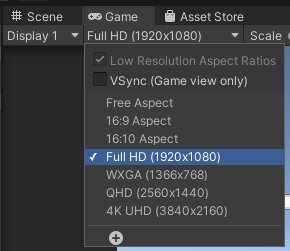
\includegraphics[width=0.3\linewidth]{rc/unity_set_ui_resolution_game}%
\hfill	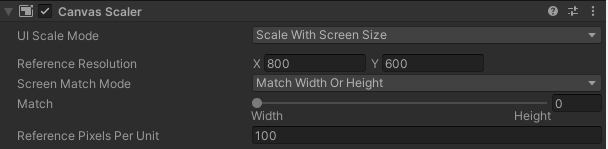
\includegraphics[width=0.6\linewidth]{rc/unity_set_ui_resolution_canvas_scaler}%
\hfill
\end{center}

\ifversionenseignant
\begin{solution}
	\begin{itemize}
		\item Créer un nouveau projet de type \texttt{3D Core}.
		\item Dans l'onglet \texttt{Game} de l'interface, cliquer sur \texttt{Free Aspect} et sélectionner une résolution, par exemple \textit{Full HD (1920x1080)}.
		\item Ajouter un \texttt{Canvas} dans la \texttt{Hierarchy}.
		\item Modifier le \texttt{Component Canvas Scaler}:
		\begin{itemize}
			\item \texttt{UI Scale Mode > Scale With Screen Size}
			\item \texttt{Reference Resolution} : faire correspondre à la résolution précédemment choisie
		\end{itemize}
	\end{itemize}

par défaut, le \texttt{Canvas} a comme propriété \texttt{Canvas > Render Mode} la valeur \texttt{Screen Space - Overlay} qui signifie que le \texttt{Canvas} va couvrir tout l'écran d'affichage (par conséquent, les propriétés du \texttt{Rect Transform} sont désactivées).
\end{solution}
\fi 


Une fois cela réalisé, nous pouvons passer à la réalisation d'un widget complexe. Pour expliquer ce terme, nous allons réaliser un agglomérat de widgets existants avec un ou plusieurs scripts pour régir le comportement global du widget.

\section{Premier widget complexe: FormattedInputField}

L'objectif de ce widget est de réaliser une zone de texte qui change de couleur selon une expression régulière particulière comme sur l'image ci-dessous, où nous avons 3 \texttt{FormattedInputField}. Ainsi, lorsque la saisie est vide (le widget de gauche), nous avons une couleur standard. La présence d'un nombre engendre une couleur (le widget au centre) et une autre couleur si l'expression régulière n'est pas présente (le widget à droite).
\begin{center}
	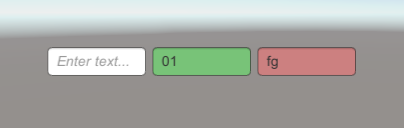
\includegraphics[width=0.4\linewidth]{rc/widget_formattetinputfield_start}
\end{center}

\ifversionenseignant
\begin{solution}
	\begin{itemize}
		\item Dans le \texttt{Canvas}, créer un \texttt{Panel} et le nommer \texttt{PanelInputFieldText}
		\begin{itemize}
			\item Définir son \textit{ancre} en \texttt{Center / Middle} pour qu'il soit placé automatiquement au centre du \texttt{Canvas}.
			\item Préciser les dimensions, par exemple\texttt{ Width = 1000} et \texttt{Height = 100}.
		\end{itemize}
	\item Dans  \texttt{PanelInputFieldText}:
	\begin{itemize}
		\item Ajouter un \texttt{ UI > Legacy > Input Field} et le renommer \textit{InputFieldText1} et modifier son \texttt{Rect Transform}:
		\begin{itemize}
			\item \texttt{Anchor Bottom Left}
			\item \texttt{Pivot X = 0 ; Pivot Y = 0}
			\item \texttt{Pos X = 0 ; Pos Y = 0; Pos Z = 0}
			\item \texttt{Width = 300, Height = 100}
		\end{itemize}
		\item Dupliquer ce \texttt{GameObject} et le renommer \textit{InputFieldText2}. Le déplacer en \texttt{Rect Tranform > Pos X = 345 ; Pos Y = 0; Pos Z = 0}.
		\item Dupliquer ce \texttt{GameObject} et le renommer \textit{InputFieldText3}. Le déplacer en \texttt{Rect Tranform > Pos X = 690 ; Pos Y = 0; Pos Z = 0}.		
		\item  Dans chaque \texttt{InputFieldText}, sélectionner le composant \texttt{Text (Legacy) }et affecter la valeur $44$ à la propriété \texttt{Character > Font Size}.
	\end{itemize}		
	\end{itemize}

Remarque : chaque \texttt{InputFieldText} contient un \texttt{Placeholder}, qui affiche par défaut le texte: "\textit{Enter text...}" (inutile de le modifier).
\end{solution}	
\fi 

Pour cela, nous vous donnons le code suivant qui vient d'un programme \texttt{C\#} basique en dehors de \texttt{Unity}:

\begin{boxcode}
\begin{csharpsansbord}
Console.WriteLine("Regex experimentation");
string regex = "[0-9]+";
string montext = "bonjour";

if (System.Text.RegularExpressions.Regex.IsMatch(montext, regex))
	Console.WriteLine("Le texte matche la regex");
else
	Console.WriteLine("le texte ne matche pas la regex");

\end{csharpsansbord}
\end{boxcode}


D'un point de vue conceptuel, nous devons suivre les étapes suivantes (vous pouvez procéder autrement, mais sans garantie de bon fonctionnement)% (si vous faites autrement, tant pis pour vous, même si cela peut fonctionner):
\begin{enumerate}
	\item Créer les attributs publics correspondant aux couleurs et les initialiser directement.
	\item Créer l'attribut de la \texttt{regex} sous forme de chaîne de caractères.
	\item Réaliser la \texttt{callback} lorsqu'on change le texte dans le champ de saisie.
	\item La couleur qu'il faut changer est celle du composant image.
\end{enumerate}

\begin{info}
Pour réaliser le dernier point, il faut bien se rappeler de la séance précédente et de la partie sur l'\texttt{Inspector} des objets en \texttt{Unity}. En effet, %si on regarde bien, 
nous avons différents \texttt{Components} pour le champs de saisie. Le \texttt{Component} qui nous intéresse est l'\textbf{image} permettant de changer l'attribut \texttt{color} pour répondre à nos conditions. Pour cela, il nous suffit, à partir du \texttt{GameObject}, de récupérer l'objet souhaité:

\begin{csharp}
Image image = gameObject.GetComponent<Image>();
\end{csharp}

J'insiste que \texttt{GetComponent} récupère le premier composant du type souhaité dans le \texttt{GameObject} courant, il existe une version permettant de récupérer tous les composants d'un type cible.
\begin{csharp}
Image[] images = gameObject.GetComponents<Image>();
\end{csharp}
\end{info}

Réaliser le widget voulu, en attachant une importance à la hiérarchie dans la structure de votre projet et aux noms que vous adoptez (harmonisation et uniformisation).

\ifversionenseignant
\begin{solution}
Associer le script \textit{FormattedInputFieldScript.cs} à chacun des \texttt{InputFieldTexts}.

\begin{boxcode}
	\begin{csharpsansbord}
using System.Collections;
using System.Collections.Generic;
using UnityEngine;
using UnityEngine.UI;
using System.Text.RegularExpressions;

// Script à associer aux GameObject de type "InputFieldText"

public class FormattedInputFieldScript : MonoBehaviour
{
	// Regex validant uniquement une suite de chiffres.
	// Modifiable dans l'Inspector
	public string m_Regex = "^[0-9]+$";
	
	// Composant InputField lié à ce GameObject
	private InputField m_InputField;
	
	// Si InputField vide
	private Color colorEmpty = Color.white;
	
	// Si texte de l'InputField ne valide pas le regex
	private Color colorError = Color.red;
	
	// Si texte de l'InputField valide le regex
	private Color colorValid = Color.green; 
	
	
	// Start is called before the first frame update
	void Start()
	{
		m_InputField = this.GetComponent<InputField>();
		if (m_InputField == null) {
			Debug.Log("[FormattedInputFieldScript] input field = nul");
		}
		
		m_InputField.onValueChanged.AddListener(delegate {
			ValueChangeCheck();
		});
		
	}
	
\end{csharpsansbord}
\end{boxcode}


\begin{boxcode}
\begin{csharpsansbord}
	// Attention : cette fonction est définie indépendamment de la méthode Start()
	// => initialiser  [m_Text] et [m_Image] dans Start() ne sert à rien
	// ==> ils sont considérés comme null dans cette fonction.
	// ===> on en fait des variables locales et le problème est réglé.
	private void ValueChangeCheck() {
		string m_Text = m_InputField.text;
		if (m_Text == null) {
			Debug.Log("[FormattedInputFieldScript] text = nul");
		}
		else {
			// Le type "string" ne supporte pas la concaténation à la Java
			// => Debug.Log("m_Text = " + m_Text); provoque des erreurs
			Debug.Log(string.Concat("m_Text = ", m_Text));
			
			Image m_Image = this.GetComponent<Image>();
			if (m_Image == null) {
				Debug.Log("[FormattedInputFieldScript] image = nul");
			}
			
			if (string.IsNullOrEmpty(m_Text)) {
				m_Image.color = this.colorEmpty;
			}
			else {
				Debug.Log(string.Concat("m_Regex = ", m_Regex));
				
				// Version fonctionnelle numéro 1
				/*
				if (Regex.IsMatch(m_Text, m_Regex)) {
					m_Image.color = colorValid;
				}
				else {
					m_Image.color = colorError;
				}
				*/
				
				// Version fonctionnelle numéro 2
// https://docs.unity3d.com/Manual/BestPracticeUnderstandingPerformanceInUnity5.html
// https://learn.microsoft.com/en-us/dotnet/api/system.text.regularexpressions.regex.match?view=net-8.0
				Regex myRegExp = new Regex(m_Regex);
				Match myMatch = myRegExp.Match(m_Text);
				if (myMatch.Success) {
					m_Image.color = colorValid;
				}
				else {
					m_Image.color = colorError;
				}
			}
		}
	}
}	
\end{csharpsansbord}
\end{boxcode}
		
\end{solution}
\fi 

\section{Widget: ComplexSlider}

Dans la section précédente, nous avions un unique \texttt{widget}. Ici, nous allons composer un \texttt{widget} complexe à partir de 3 \texttt{widgets} basiques. Pour cela, nous allons réaliser des curseurs complexes en composant un \texttt{Text} qui servira de \texttt{Label}, d'un \texttt{Slider} basique et d'un \texttt{InputTextField} sur les nombres pour visualiser la valeur du \texttt{Slider} et/ou la modifier manuellement. Ci-dessous, vous avez une image qui illustre deux \texttt{ComplexSliders} pour choisir des coordonnées \texttt{(x,y)}.

\begin{center}
	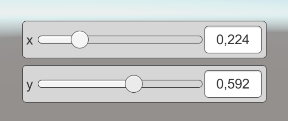
\includegraphics[width=0.5\linewidth]{rc/widget_complexslider_demo}
\end{center}

\begin{info}
Généralement, un widget complexe doit avoir un \texttt{Panel} à la base pour servir de fond visuel, que vous opacifierez par défaut et qui permet de hiérarchiser les 3 sous-\texttt{widgets} le composant.
\end{info}

Vous devez réaliser un tel composant puis réaliser un unique script qui gouverne tous les aspects comportementaux. En particulier, lorsqu'une valeur est modifiée, cela impacte l'autre \texttt{widget} pour avoir toujours une cohérence entre le champ de saisie et le \texttt{Slider} basique.

Pour cela, nous allons exploiter la hiérarchie de notre \texttt{widget}. Il existe deux mécaniques pour retrouver les enfants:
\begin{enumerate}
	\item \textit{via} les fonctions de recherche basées sur leur nom,
	\item \textit{via} les mécaniques de recherche sur un type souhaité.
\end{enumerate}
Réfléchissez sur les avantages et inconvénients des deux mécaniques en lisant la documentation associée à ces familles de fonctions: \url{https://docs.unity3d.com/ScriptReference/GameObject.html}.
En particulier, que se passe-t-il si plusieurs objets sont du même type? Ou si l'utilisateur modifie le nom d'un sous-\texttt{widget} ?

\ifversionenseignant
\begin{solution}
\subsection{Création du Panel}
\begin{itemize}
	\item Dans le \texttt{Canvas} principal, créer un nouveau \texttt{Panel} et le nommer \textit{PanelComplexSlider1}. 
	\item Définir son \texttt{ancre} en \texttt{Center / Middle}.
	\item  Préciser les dimensions, par exemple \texttt{Width = 1000 et Height = 100}. \item Déplacer \textit{PanelComplexSlider1} en \texttt{Pos X = 0; Pos Y = -200; Pos Z = 0}.	
	\item Dans \textit{PanelComplexSlider1}, créer
	\begin{itemize}
		\item un  \texttt{Text avec UI > Legacy > Text} renommé \textit{Text}
		\begin{itemize}
			\item \texttt{Rect Transform}
			\begin{itemize}
				\item \texttt{Anchor = bottom left}
				\item \texttt{Pivot : X = 0 ; Y = 0}
				\item \texttt{Pos X = Pos Y = Pos Z = 0}
				\item \texttt{Width = 40 : Height = 100}				
			\end{itemize}
		    \item Text
		    \begin{itemize}
		    	\item \texttt{Text = x}
		    	\item \texttt{Font Size = 44}
		    	\item \texttt{Paragraph > Alignment = middle / center}
		    \end{itemize}
		\end{itemize}
		\item un \texttt{Slider} avec \texttt{UI > Slider}
		\begin{itemize}
			\item \texttt{Rect Transform}
			\begin{itemize}
				\item \texttt{Anchor = bottom left}
				\item \texttt{Pivot : X = 0.5 ; Y = 0.5}
				\item \texttt{Pos X = 450 ; Pos Y = 50 ; Pos Z = 0}
				\item \texttt{Width = 700 : Height = 60}				
			\end{itemize}
			\item Enfant \texttt{Handle Slide Area > Handle} : dans \texttt{Rect Transform}, modifier la propriété \texttt{Height} pour que la poignée du \texttt{Slider} dessine un joli cercle, égale à la hauteur du \texttt{Slider} : $60$.
		\end{itemize}
		\item un \texttt{Input Field} \textit{InputFieldComplexSlider} avec \texttt{UI > Legacy > Input Field}
		\begin{itemize}
			\item \texttt{Rect Transform}
			\begin{itemize}
				\item \texttt{Anchor = bottom left}
				\item \texttt{Pivot : X = 0 ; Y = 0}
				\item \texttt{Pos X = 830 ; Pos Y = 20 ; Pos Z = 0}
				\item \texttt{Width = 160 : Height = 60}				
			\end{itemize}
			\item Enfant \texttt{PlaceHolder > Text} : effacer le texte par défaut \textit{Enter text...}
			\item Enfant \texttt{Text (Legacy)} : propriété \texttt{Text}
			\begin{itemize}
				\item \texttt{Font Size = 24}. \textbf{ATTENTION} : le texte ne s'affiche pas si une taille de police est trop importante.
				\item \texttt{Paragraph > Alignment = middle / center}
			\end{itemize}
		\end{itemize}
	\end{itemize}
	
\end{itemize}

\subsection{Script de PanelComplexSlider1}

\begin{boxcode}
\begin{csharpsansbord}
using System.Collections;
using System.Collections.Generic;
using UnityEngine;
using UnityEngine.UI;
using UnityEngine.EventSystems;

public class ComplexSliderScript : MonoBehaviour 
{
	public Slider m_Slider;
	public InputField m_InputField;
	
	// Start is called before the first frame update
	void Start()
	{
		m_Slider = gameObject.GetComponentInChildren<Slider>();
		m_InputField = gameObject.GetComponentInChildren<InputField>();
		
		Debug.Log("Slider found: " + m_Slider  + " name: " + m_Slider.name);
		Debug.Log("Field found: " + m_InputField + "name: " + m_InputField.name);
		
		m_Slider.onValueChanged.AddListener(UpdateValueFromFloat);
		m_InputField.onEndEdit.AddListener(UpdateValueFromString);
	}
	
	// Update is called once per frame
	void Updte()	{ }
	
	public void UpdateValueFromFloat(float value)
	{
		Debug.Log("float value changed: " + value);
		if (m_InputField) { m_InputField.text = value.ToString(); }
		else Debug.Log("m_InputField not found");
	}
	
	public void UpdateValueFromString(string value)
	{
		Debug.Log("string value changed: " + value);
		try
		{
			float ff = float.Parse(value);
			if (m_Slider && m_Slider.value != ff) { m_Slider.value = ff; }
		}
		catch(System.Exception e) {
			Debug.Log("error: " + e);
		}
	}
}
		
\end{csharpsansbord}
\end{boxcode}		

\end{solution}
\fi 

\section{Exporter son travail}

Bravo, vous avez fait le plus gros. Demander à l'enseignant  qu'il vérifie votre développement ou critique vos noms et autres petits détails.

\subsection{Préfabriqué}
L'intéret de développer un widget est de pouvoir le réutiliser plusieurs fois sans devoir faire plusieurs manipulations identiques ou des \texttt{copier-coller}. Pour cela, \texttt{Unity} a la possibilité de créer des \texttt{Préfabs}, une sorte de sauvegarde de votre réalisation au sein d'un projet.

La procédure est assez simple: lorsque vous avez fini un \texttt{widget} qui n'a pas de dépendance extérieure, c'est-à-dire que le \texttt{widget} est autonome (sinon les dépendances risquent aussi d'être sauvegardées): il suffit de glisser le \texttt{GameObject} de la hiérarchie à la zone des \texttt{Assets}. Ainsi l'icône du \texttt{Gameobject} devient bleue! C'est ainsi qu'on sait qu'il s'agit d'un \texttt{Prefab}.


\begin{info}
Lorsque vous sélectionnez un \texttt{Prefab} dans la zone des \texttt{Assets}, vous avez un nouveau bouton dans l'\texttt{Inspecteur} qui vous permet de modifier ce \texttt{Prefab}.
\begin{center}
	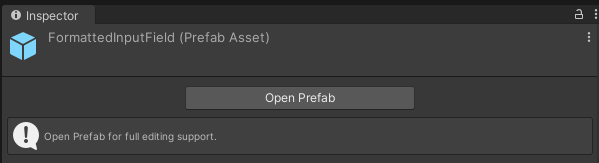
\includegraphics[width=0.5\linewidth]{rc/unity_set_ui_open_prefab}
\end{center}
\end{info}

\begin{attention}
Quand vous modifiez un \texttt{Prefab}, vous êtes dans un environnement particulier. Il est essentiel de revenir au plus vite dans le mode standard, en particulier pour sauvegarder et ainsi éviter des petits problèmes. 

Pour quitter, il faut cliquer sur le bouton "Retour" (noté par $'<'$) au niveau de la hiérarchie.
\begin{center}
	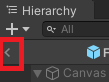
\includegraphics[width=0.3\linewidth]{rc/unity_set_ui_close_prefab}
\end{center}
\end{attention}

Réaliser des \texttt{Prefabs} de vos widgets en les ayant nettoyés si besoin AVANT! Ensuite, instancier pour expérimenter deux ou trois de vos \texttt{Prefabs}. Pour cela, il suffit de glisser votre \texttt{Prefab} depuis l'\texttt{Assert} vers la vue 3D ou la hiérarchie à l'endroit souhaité.

\ifversionenseignant
\begin{solution}
Un \texttt{Prefab} est un container représentant la sauvegarde d'un \texttt{Component}, que l'on peut réutiliser dans d'autres projets.

Il suffit de sélectionner le composant qui nous intéresse : ici, \textit{PanelComplexslider1}, et de le déplacer dans le \texttt{Project}.\\

\textbf{Attention} : veiller à ce que ce composant n'ait pas de dépendance extérieure, sinon ces dernières seront également sauvegardées dans le \texttt{Prefab}.\\

Remarque : si l'on sélectionne ce \texttt{Prefab}, l'\texttt{Inspector} affiche un bouton \texttt{Open} qui modifie l'interface principale pour lister uniquement la hiérarchie de ce \texttt{Prefab}. Pour revenir à la hiérarchie complète, on clique sur le symbole '\texttt{<}' à gauche du nom du \texttt{Prefab} dans la hiérarchie.

\paragraph{Dupliquer un Prefab et le modifier}

La duplication est simple : on sélectionne le \texttt{Prefab} dans le \texttt{Project} et on le déplace dans la fenêtre d'affichage ou dans la hiérarchie. Prendre soin de l'insérer comme enfant du \texttt{Canvas}.

% [XS] 2024-03-29 : la remarque ci-dessous n'est plus vraie, je ne me souviens plus
% comment j'avais obtenu ce comportment.
%\textbf{Attention} : le \texttt{Prefab} original n'est pas dupliqué dans le \texttt{Project} : une seconde instance de ce \texttt{Prefab} a simplement été créée.
%Cela implique que toute modification d'une instance se répercute automatiquement sur les autres (en d'autres termes, les instances partagent les mêmes attributs.
%Par exemple, modifier le nom "\textit{x}" à côté d'un \texttt{Slider} en "\textit{y}" sur l'une des instances et noter la modification de l'autre. 
%En revanche, les scripts fonctionnent de manière indépendante entre les instances, comme s'il s'agissait de \texttt{GameObject} différents.\\

Si l'on veut modifier un attribut d'un \texttt{Prefab}, on peut sélectionner ce dernier dans le \texttt{Project}, puis faire un copier-coller. Un \texttt{Prefab} identique au précédent est créé (avec un nouveau nom) et on peut modifier ses attributs, indépendamment du \texttt{Prefab} original.
	
\end{solution}
\fi 
	

\subsection{Export}

Maintenant que vous avez la possibilité de sauvegarder et réutiliser votre production au sein d'un projet, il est fréquent de devoir les exporter pour les utiliser dans d'autres projets. 
Pour cela, il faut exporter des \texttt{Prefabs} dont vous connaissez les dépendances, en sélectionnant votre \texttt{Prefab} dans les \texttt{Assets} et en faisant un clique droit dessus (attention, on vous demande de tester l'export d'un widget dans un premier temps, puis plusieurs widgets dans un second temps afin que vous compreniez les dépendances). Dans le menu contextuel, sélectionner \texttt{'Export Package\ldots'}.

Dans la nouvelle fenêtre, vous devez sélectionner les bonnes dépendances de votre widget. En particulier, \texttt{Unity} sélectionne par défaut tous les scripts sans distinction, car il n'arrive pas à calculer les dépendances correctement. Vous devez donc sélectionner les bonnes dépendances de scripts manuellement. Puis, cliquez sur le bouton \texttt{Export...} pour sauvegarder le package \texttt{Unity}.

\begin{center}
\hfill 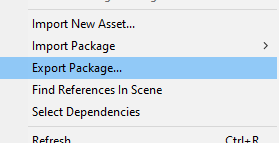
\includegraphics[width=0.35\linewidth]{rc/unity_set_ui_export_package}
\hfill 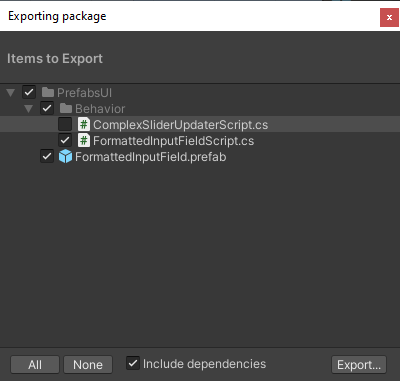
\includegraphics[width=0.5\linewidth]{rc/unity_set_ui_export_prefab_deps}
\hfill 
\end{center}

\ifversionenseignant
\begin{solution}
\begin{itemize}
	\item Sélectionner un \texttt{Prefab} dans l'onglet \texttt{Project}
	\item clique droit : sélectionner \texttt{Export...} et ne cocher que les dépendances nécessaires:
	\begin{itemize}
		\item le \texttt{Prefab} lui-même;
		\item le script \textit{ComplexSliderScript.cs}
	\end{itemize}
	\item puis valider l'export en précisant son nom, par exemple \textit{MyPrefabComplexSlider} : un fichier du nom \textit{MyPrefabComplexSlider.unitypackage} est créé.
\end{itemize}
\end{solution}
\fi 


\subsection{Import}

Pour tester nos paquets \texttt{Unity} créés à l'étape précédente, c'est très simple! Il suffit de créer un nouveau projet \texttt{Unity} et glisser votre fichier \texttt{.unitypackage} dans les \texttt{Assets}, puis se laisser guider par le menu.

\begin{info}
Une alternative consiste  à faire juste un clique droit dans la zone des \texttt{Assets} et cliquer sur l'import d'un paquet personnalisé.
\end{info}

Votre widget est prêt à l'emploi. La mécanique des \texttt{Unity packages} est l'une des façons de se partager le travail lorsqu'on est plusieurs sur un même projet et que cela s'y prête bien. 

\ifversionenseignant
\begin{solution}
	\begin{itemize}
		\item Créer un nouveau projet \texttt{Unity}
		\item Dans le menu principal, cliquer sur \texttt{Assets > Import Package > Custom Package...}
		\item Sélectionner \textit{MyPrefabCmplexslider.unitypackage} (on peut sélectionner tout ou partie du package)
		\item Cliquer sur \texttt{Import} après la sélection
		\item Un \texttt{GameObject} nommé \textit{PanelComplexSlider1} apparaît dans \texttt{Project > Assets}.		
		\item Il n'est pas directement visible : créer un \texttt{Canvas} et intégrer \textit{PanelComplexSlider1} comme son enfant.		
		\item \texttt{PanelComplesSlider} est un objet 3D ! Modifier sa position pour le "coller" au \texttt{Canvas (Rect Transform > Pos Z = 0)}.		
		\item Passer dans le \texttt{Game View} et tester le \texttt{ComplexSlider} $\Rightarrow$ penser à remettre la résolution du projet original, le \texttt{Slider} risque de ne pas être adapté à la résolution du nouveau projet...		
	\end{itemize}

\end{solution}
\fi 


\section{Toujours plus loin}

\subsection{Des Prefabs partout !}
Reprendre votre TP précédent ou un nouveau projet qui exploite vos nouveaux widgets, histoire de voir une application complète et comprendre que votre \texttt{Prefab} doit bien être autonome pour embarquer uniquement son comportement intrinsèque!

\ifversionenseignant
\begin{solution}
On peut reprendre le projet sur le système solaire et vérifier que le \texttt{ComplexSlider} s'intègre correctement (l'interface commence à être "bouchée" mais bon...)	
\end{solution}
\fi 

\subsection{Retour sur la multi-résolution}
En reprenant l'hyperlien cité en introduction, vérifier que les \textit{ancres} des éléments du \texttt{Canvas} sont bien définies puis jouer avec le composant \texttt{Canvas Scaler} pour tester le positionnement de ces éléments. 

Tester également les résolutions proposées dans le \texttt{GameView}. Enfin, créer une résolution personnalisée (imiter un mode "\textit{Portrait}" par exemple) et vérifier si les widgets sont toujours positionnés correctement.

\ifversionenseignant
\begin{solution}
	\href{ https://docs.unity3d.com/2020.1/Documentation/Manual/HOWTO-UIMultiResolution.html}{Documentation multiresolution}. \\
	
La documentation du \texttt{Canvas Scaler} permet de jouer sur plusieurs paramètres, notamment :
\begin{itemize}
	\item \texttt{Constant Pixel Size} : tailles indépendantes de la résolution.
	\item \texttt{Scale With Screen Size} : à partir de la \texttt{Reference Resolution}, les dimensions des \texttt{widgets} s'adaptent en fonction de la largeur ou de la hauteur du \texttt{Canvas} (valeur entre 0 et 1).
	\item \texttt{Constant Physical Size} : s'appuie sur une unité physique pour recalculer les dimensions.
\end{itemize}

De plus, dans l'onglet \texttt{Resolution} qui permettait de sélectionner "\textit{Full HD}" (entre autres), on peut créer sa propre résolution, pour imiter le mode \textit{Paysage} : essayer par exemple \textit{1080x1920} pour vérifier les dimensions et la disposition des \texttt{widgets}.

\end{solution}
\fi 


\subsection{Orientation du Canvas}
À partir du lien \href{https://docs.unity3d.com/2022.3/Documentation/Manual/UICanvas.html}{UICanvas}, expérimenter les modes de rendu "\texttt{Screen Space - Camera}" et "\texttt{World Space}" pour modifier l'orientation et la position du \texttt{Canvas} et de ses enfants.

\ifversionenseignant
\begin{solution}
On veut faire pivoter le \texttt{Canvas} pour obtenir le même effet que celui montré dans l'hyperlien.

\begin{itemize}
	\item Sélectionner le \texttt{Canvas} dans la hiérarchie
	\begin{itemize}
		\item Propriété \texttt{Render Mode = World Space} => \texttt{Unity} se plaint si aucune caméra n'est associée à ce mode
		\item Propriété \texttt{Event Camera} : faire glisser une des caméras de la scène (par exemple \textit{Main Camera} dans cette propriété
\end{itemize}		
	\item Composant \texttt{Rect Transform}
	\begin{itemize}	
	\item \texttt{Pos Z} : modifier cette valeur pour éloigner le \texttt{Canvas} de la caméra;
	\item \texttt{Rotation} : modifier la valeur sur chacun des axes pour observer différents effets.
\end{itemize}		
\end{itemize}

Remarques:
	\begin{itemize}	
	 \item On peut modifier la rotation de chaque enfant du \texttt{Canvas} indépendamment des autres.
	 \item Si on utilise la valeur \texttt{Canvas > Render Mode = Screen Space - Camera} (toujours avec la caméra associé au \texttt{Canvas}), le positionnement du \texttt{Canvas} (\textit{i.e.} \texttt{Component Rect Transform}) est désactivé. Mais on peut toujours modifier le positionnement de ses enfants.
	
\end{itemize}


\end{solution}
\fi 
\end{document}
